\subsection{Aggiungi nuovo LLM}

\begin{figure}[H]
    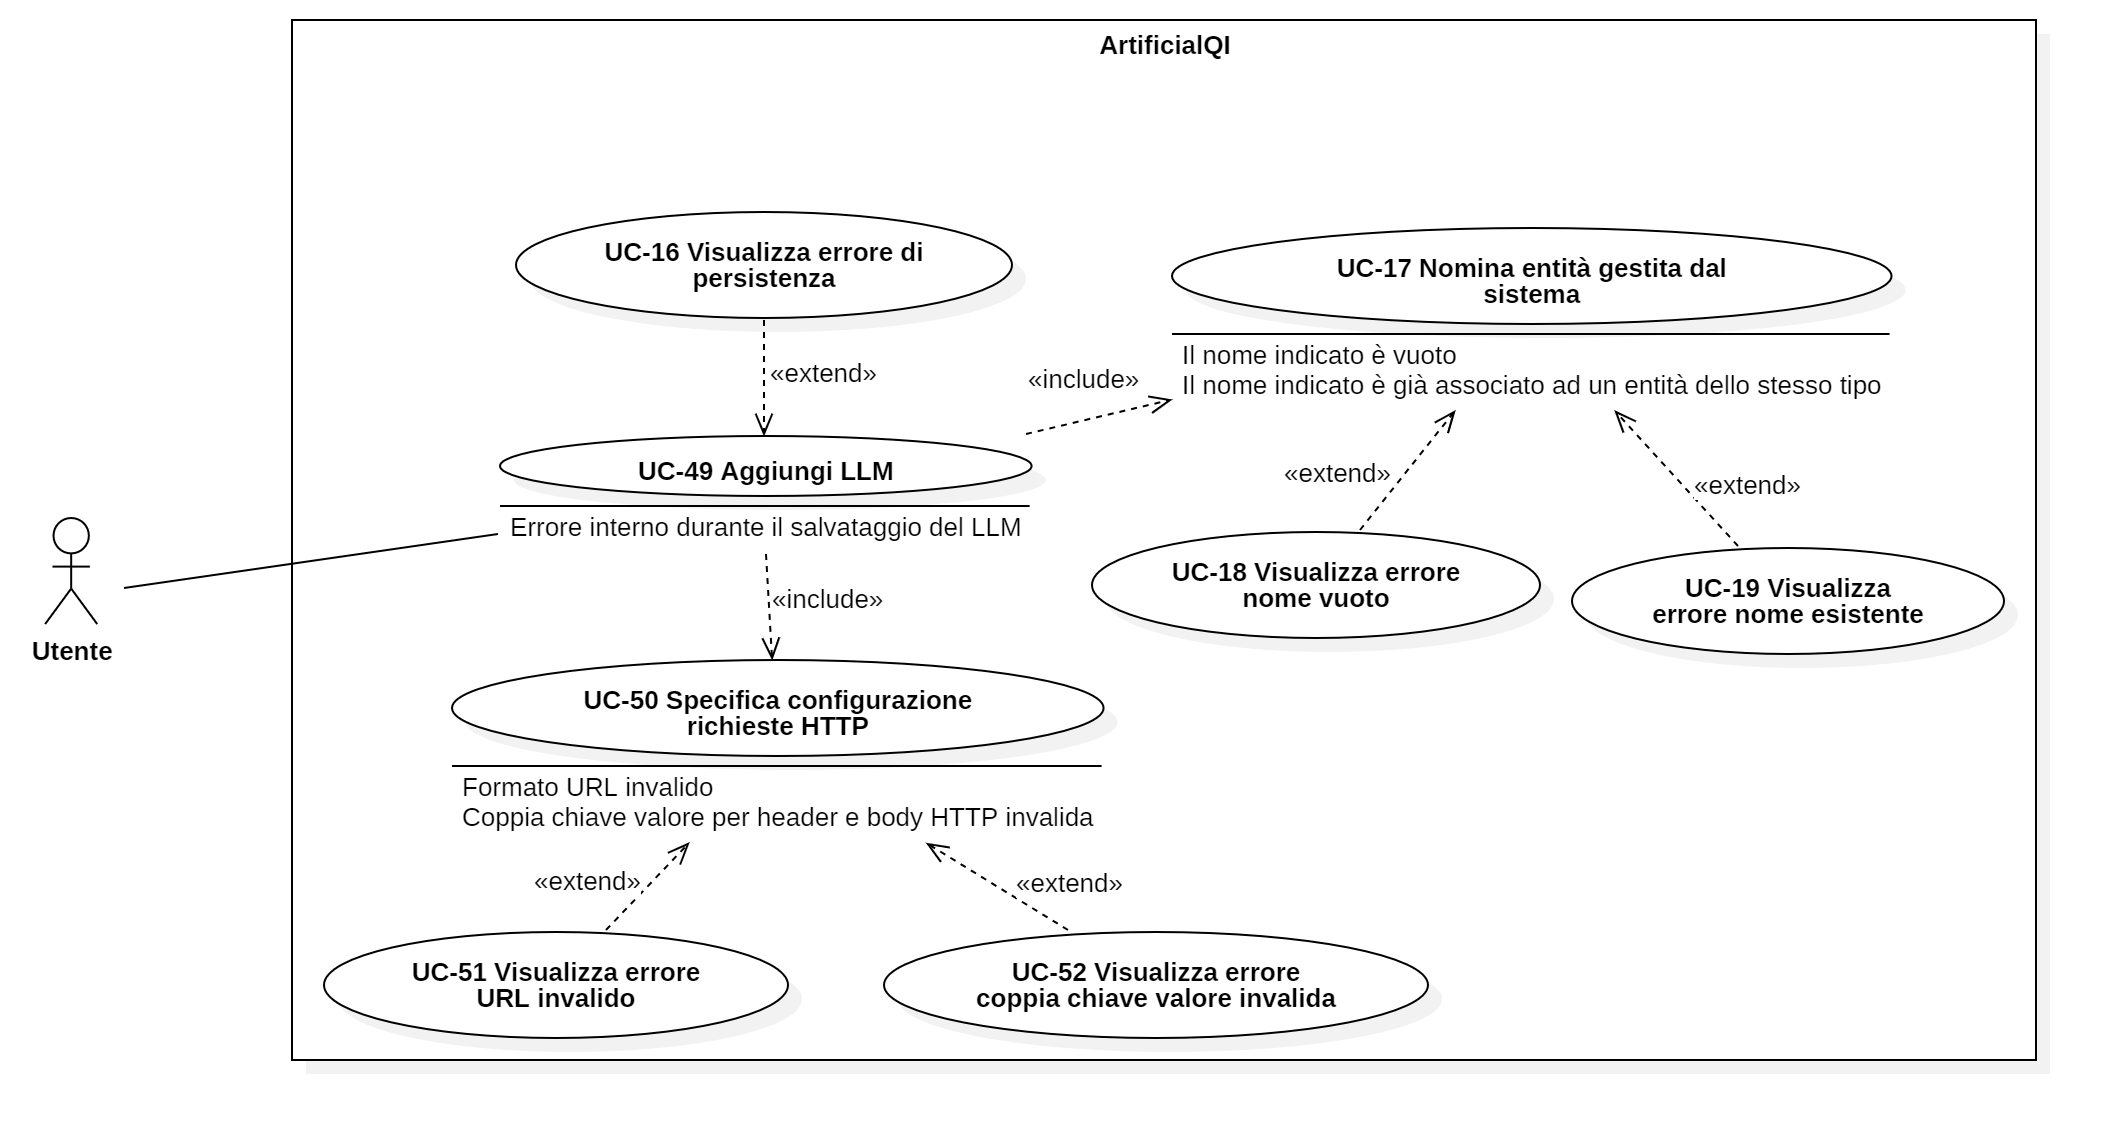
\includegraphics[scale=0.45]{Sezioni/UseCase/Immagini/AggiungiLLM.png}
    \caption{Diagramma aggiungi nuovo LLM.}
\end{figure}

\begin{usecase}{UC-46}{Aggiungi LLM} 
    \label{uc:UC-46}
    
    \req{\hyperref[ru:RUF-6]{RUF-6}} 

    \pre{ 
        \item L'utente sta visualizzando gli LLM salvati \hyperref[uc:UC-52]{UC-52}
    } 
    
    \post{
        \item Viene aggiunto un nuovo LLM nel sistema
    }

    \actor{Utente} 

    \trigger{L'utente vuole aggiungere un nuovo LLM} 

    \inc{\hyperref[uc:UC-14]{UC-14}, \hyperref[uc:UC-47]{UC-47}}

    \base{} 

    \scenario{ 
        \item L'utente richiede di aggiungere un nuovo LLM 
                    
        \item  L'utente specifica la configurazione necessaria per realizzare le chiamate HTTP verso l'LLM seguendo \hyperref[uc:UC-47]{UC-47}
             
        \item Viene richiesta l'assegnazione di un nome per il nuovo LLM seguendo \hyperref[uc:UC-14]{UC-14}

        \item Il sistema salva il nuovo LLM 
    } 

    \subscenario{ 
        \item[4.1] Errore durante il salvataggio dell'LLM:
        \begin{itemize}
            \item \hyperref[uc:UC-13]{UC-13}
        \end{itemize}
    } 
  \end{usecase}
  
  \begin{usecase}{UC-47}{Specifica configurazione richieste HTTP} 
    \label{uc:UC-47}

    \req{} 
    
    \pre{ 
        \item L'utente sta aggiungendo  un nuovo LLM
    } 
    
    \post{ 
        \item Il sistema ottiene la configurazione da utilizzare per le comunicazioni HTTP con l'LLM
    }
    
    \actor{} 
    
    \trigger{
        L'utente deve specificare la configurazione per le richieste HTTP all'LLM
    } 

    \inc{} 
    
    \base{} 

    \scenario{
        \item L'utente specifica l'URL relativo all'LLM
        
        \item L'utente specifica zero o più coppie chiave-valore da utilizzare nell'header HTTP delle richieste verso l'LLM
        
        \item L'utente specifica zero o più coppie chiave-valore da utilizzare nel body delle richieste HTTP verso l'LLM
         
        \item L'utente specifica la chiave da associare alle domande da porre all'LLM
         
        \item L'utente specifica la chiave per estrarre le risposte generate dall'LLM dalla risposta HTTP
    } 
    
    \subscenario{ 
        \item[1.1] Formato dell'URL inserito invalido:
        \begin{itemize}
            \item \hyperref[uc:UC-48]{UC-48}
        \end{itemize}
        \item[2.1] L'utente specifica una coppia chiave-valore invalida:
        \begin{itemize}
            \item \hyperref[uc:UC-49]{UC-49}
        \end{itemize}
        \item[3.1] L'utente specifica una coppia chiave-valore invalida:
        \begin{itemize}
            \item \hyperref[uc:UC-49]{UC-49}
        \end{itemize}
    } 
\end{usecase}

\begin{usecase}{UC-48}{Visualizza errore URL invalido} 
    \label{uc:UC-48}

    \req{} 

    \pre{ 
        \item Il formato dell'ULR è invalido
    } 

    \post{ 
        \item L'utente è a conoscenza che l'URL fornito è in un formato invalido
    }

    \actor{} 

    \trigger{
        Il sistema fallisce la validazione di un URL specificato dall'utente
    } 

    \inc{} 

    \base{} 

    \scenario{
        \item Il sistema mostra un messaggio di errore in cui viene indicato che l'URL è invalido
    } 

    \subscenario{} 
\end{usecase}

\begin{usecase}{UC-49}{Visualizza errore coppia chiave-valore invalida} 
    \label{uc:UC-49}

    \req{} 

    \pre{ 
        \item La chiave o il valore sono vuote o composte da soli spazi
    } 

    \post{ 
        \item L'utente è a conoscenza che la coppia chiave-valore è invalida
    }

    \actor{} 

    \trigger{
        Il sistema fallisce la validazione di una coppia chiave-valore specificata dall'utente
    } 

    \inc{} 

    \base{} 

    \scenario{
        \item Il sistema mostra un messaggio di errore in cui viene indicato che una coppia chiave-valore non può contenere componenti vuoti
    } 

    \subscenario{} 
\end{usecase}
